\documentclass[12pt]{article}
\usepackage{geometry}                % See geometry.pdf to learn the layout options. There are lots.
\geometry{letterpaper}                   % ... or a4paper or a5paper or ... 
%\geometry{landscape}                % Activate for for rotated page geometry
\usepackage[parfill]{parskip}    % Activate to begin paragraphs with an empty line rather than an indent
\usepackage{daves,fancyhdr,natbib,graphicx,dcolumn,amsmath,lastpage,url}
\usepackage{amsmath,amssymb,epstopdf,longtable}
\usepackage[final]{pdfpages}
\DeclareGraphicsRule{.tif}{png}{.png}{`convert #1 `dirname #1`/`basename #1 .tif`.png}
\pagestyle{fancy}
\lhead{CE 5364 -- Groundwater Transport Phenomena }
\rhead{FALL 2024}
\lfoot{ES1}
\cfoot{}
\rfoot{Page \thepage\ of \pageref{LastPage}}
\renewcommand\headrulewidth{0pt}



\begin{document}
\begin{center}
{\textbf{{ CE 5364 Groundwater Transport Phenomena } \\ {Exercise Set 1}}}
\end{center}

\section*{\small{Exercises}}
\begin{enumerate}
\item 

A sand column has the following characteristics\footnote{Problem 2-3, pg. 578 in Bedient, et. al.}:
%$$ K = 10^{-4} \frac{cm}{s} \\ A = 75 cm^{2} \\ \frac{dh}{dl} = 0.01 \\ n = 0.20$$
\begin{equation}
  \begin{aligned}
    K = 10^{-4} \frac{cm}{s}; & ~~A = 75 cm^{2}; & ~~\frac{dh}{dl} = 0.01; & ~~n = 0.20 
  \end{aligned}
\end{equation}

Determine:
\begin{enumerate}
\item Sketch the system.
\item The discharge velocity.
\item The seepage velocity.
\item The volumetric flow rate through the column.
\end{enumerate}

\item Three geologic formations overlie one another with the characteristics listed below.\footnote{Problem 2-12, pg. 579 in Bedient, et. al.}

\begin{equation}
  \begin{aligned}
b_1 = & 50~ft &K_1 =   0.0002 \frac{ft}{s} \\ 
b_2 = & 20~ft &K_2 = 0.000005 \frac{ft}{s} \\
b_3 = &210~ft &K_3 =    0.001 \frac{ft}{s} \\
  \end{aligned}
\end{equation}

A constant velocity vertical flow field exists across the three formations.
The hydraulic head at the top of the formations (top of formation 1) is 33 feet.  The hydraulic head at the bottom of the formations (bottom of formation 3) is 21 feet.

Determine:
\begin{enumerate}
\item Sketch the system.
\item The hydraulic head at the internal boundary between formation 1 and 2.
\item The hydraulic head at the internal boundary between formation 2 and 3.
\item Approximate time for a tracer to flow (vertically) through the three layers if the porosities $n_1$, $n_2$, and $n_3$ are 0.30,0.42, and 0.35, respectively
\end{enumerate}

\clearpage

\item Figure \ref{fig:plumemap} below shows a piezometric map for a shallow sand aquifer.\footnote{Problem 2-8, pg. 578 in Bedient, et. al.}  The hydraulic conductivtiy is estimated to be $1.5 \times 10^{-2}~\frac{cm}{s}$, the saturated thickness is 40 feet, and the effective porosity is 0.3.

\begin{figure}[h!] %  figure placement: here, top, bottom, or page
   \centering
   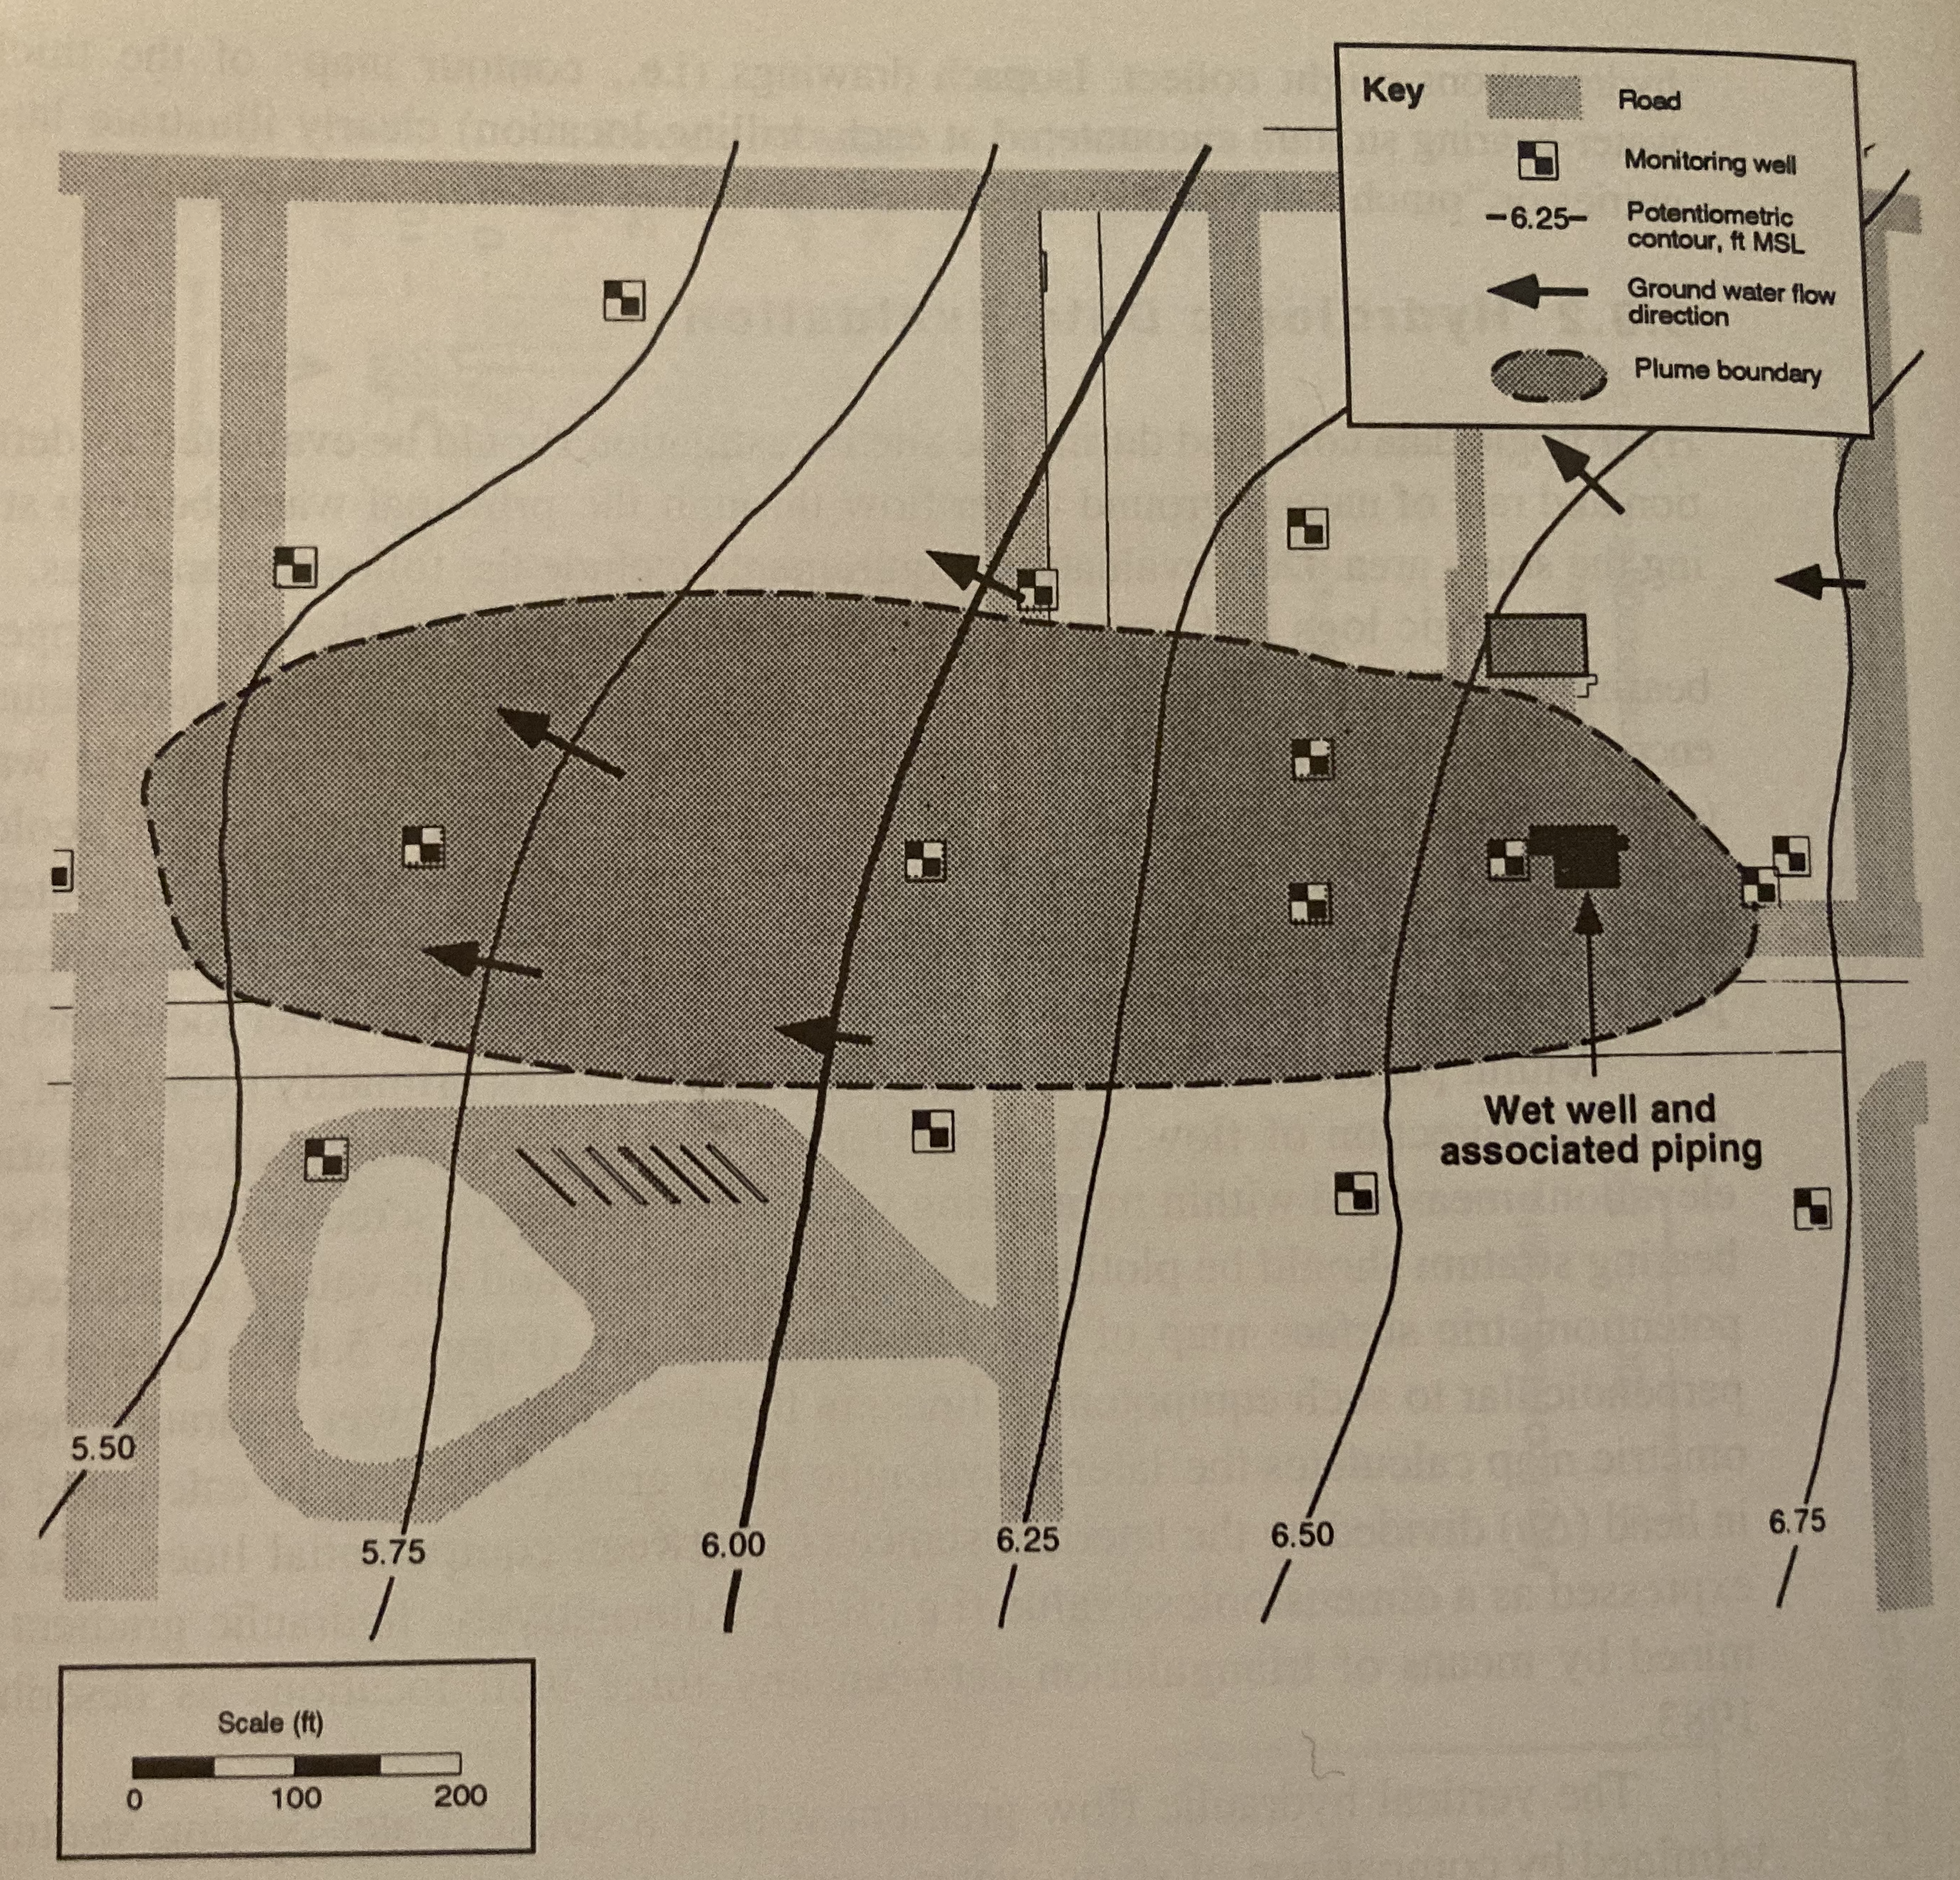
\includegraphics[width=4.5in]{Fig5.18.png} 
   \caption{Plume Map (plan view)}
   \label{fig:plumemap}
\end{figure}

Determine:
\begin{enumerate}
\item Which well is expected to be the most contaminated.
\item The groundwater velocity and seepage velocity across the plume.
\item The duration that the source has been contaminating the aquifer (neglect dispersion, diffusiom, and adsorption).
\item The flow rate across the plume.
\item An explaination for contamination upgradient of the source zone.
\end{enumerate}

\end{enumerate}
\end{document}  